\documentclass[12pt]{revtex4}
\usepackage{ulem}
\usepackage{url}
\usepackage{epsfig}
\usepackage{graphicx,color}% Include figure files
\usepackage{epstopdf}
\DeclareGraphicsRule{.tif}{png}{.png}{`convert #1 `basename #1
.tif`.png}
\usepackage[psamsfonts]{amssymb}
\usepackage{amsmath}
\usepackage{indentfirst}
%\usepackage{cite}

\newcommand{\be}{\begin{equation}}
\newcommand{\ee}{\end{equation}}
\newcommand{\ba}{\begin{eqnarray}}
\newcommand{\ea}{\end{eqnarray}}

\begin{document}
\title{\large Given Enough Eyeballs, All Bugs Are Shallow? \\ Revisiting Eric Raymond with Bug Bounty Programs}

\author{Thomas Maillart}
\email{maillart@berkeley.edu}
\affiliation{UC Berkeley, Berkeley, USA}

\author{Mingyi Zhao}
%\email{}
\affiliation{The Pennsylvania State University, University Park, USA}

\author{Jens Grossklags}
\affiliation{The Pennsylvania State University, University Park, USA}

\author{John Chuang}
\affiliation{UC Berkeley, Berkeley, USA}




\date{\today}


\begin{abstract}
\vspace{1cm}
Bug bounty programs offer a modern way for organizations to crowdsource their software security, and for security researchers to be fairly rewarded for the vulnerabilities they find. However, little is known on the incentives set by bug bounty programs -- how they drive engagement and new bug discoveries. This article provides an empirical investigation of the strategic interactions among the managers and participants of bug bounty programs, as well as the intermediation by bug bounty platforms. We find that for a given bug bounty program, each security researcher can only expect to discover a bounded number of bugs. This result offers a validation step to a theory brought forth early on by Brady et al. \cite{brady1999murphy}, which proposes that each security researcher inspecting a piece of software offers a unique environment of skills and mindset, which is amenable to the discovery of bugs that others may not be able to uncover. Bug bounty programs indeed benefit from the engagement of large crowds of researchers. Conversely, security researchers benefit greatly from searching for bugs in multiple bug bounty programs. However, we find that following a strong front-loading effect, newly launched programs attract researchers at the expense of older programs: the probability of finding bugs decays as $\sim 1/t^{0.4}$ after the launch of a program, even though bugs found later yield on average higher rewards. Our results lead us to formulate 3 recommendations for organizing bug bounty programs and platforms: (i) organize enrollment, mobility and renewal of security researchers across bounty programs, (ii) highlight and organize programs for front-loading, and (iii) organize fluid market transactions to reduce uncertainty and thus reduce incentives for security researchers to sell on the black market.




\end{abstract}

\maketitle

%\section{Introduction}
\label{sec:intro}
Software security is a hard problem, which requires automatic and human testing....\\

Crowdsourcing has become a popular way to find solutions to {\it hard problems}, such as sorting galaxies \cite{smith2013introduction}, or folding proteins \cite{khatib2011algorithm} for the sake of science, or to recognize words from books digitalized with low quality \cite{von2003captcha} and to solve big data problems \cite{narayanan2011link}. Even hard mathematical problems get addressed on open collaboration platforms \cite{gowers2009massively,cranshaw2011polymath}.\\

Finding software bugs and vulnerabilities has been one of the most long-standing challenges in computer science \cite{}, and similarly, crowdsourcing has been suggested over the last decade as a way to efficiently cope with software cybersecurity, through a number mechanisms, such as vulnerability brokerage \cite{camp2004pricing}, markets \cite{schechter2002buy} and auctions, with their presumed incentives, strengths and weaknesses \cite{ozment2004bug}.\\

Recently, however, ``bug bounty" platforms, essentially focused on crowdsourcing software vulnerabilities, have appeared and rapidly developed \cite{zhao2014exploratory,zhao2015empirical}. These online platforms offer both an infrastructure and play the role of {\it trusted third party} (TTP) between organizations (i.e., mainly Internet companies) and security researchers willing to search and submit the vulnerabilities they find.\\

As markets of some sort, as we shall describe more in details later, these platforms inform on transactions occurring between organizations and security researchers, and thus, they are thought to reveal the {\it true value} of vulnerabilities. They also provide empirical evidence on the economic behaviors of the parties involved (at least on the publicly facing parts of platform).\\

In this paper, we recognize the visionary theoretical propositions made more than 10 years ago by pioneering researchers in economics of information security \cite{schechter2002buy,ozment2004bug}, and we confront and enrich these propositions with empirical evidence.\\

In particular, we find that indeed the bug bounty platform studied here (i.e., HackerOne) works essentially as a {\bf (reverse?)} Dutch auction \cite{}. (we cannot exclude that the designers of the platform got inspired by the article published in 2005 \cite{ozment2004bug}). There are however a number of differences and refinements from the theory, which can be rationalized by business and organization contingencies. Also, our results provide a more accurate picture of challenges faced by researchers when engaging in bug bounties (i.e., the St. Petersburg paradox of bug bounty hunting), and the consolidation of monetary rewards over several bug bounty programs and how new bug bounty programs suddenly shift incentives.\\

This article is organized as follows. Related research is presented in Section \ref{sec:related}. Important features of the data set used here is detailed in Section \ref{sec:data}. We then introduce the main mechanism driving vulnerability discovery in Section \ref{sec:method}. Results are presented and discussed in respectively Sections \ref{sec:results} and \ref{sec:discussion}. We finally in conclude in Section \ref{sec:conclusion}.
%\input{sections/background}
%\input{sections/methods}
\section{Introduction}
\label{sec:intro}
Software security is a hard problem, which requires automatic and human testing....\\

Crowdsourcing has become a popular way to find solutions to {\it hard problems}, such as sorting galaxies \cite{smith2013introduction}, or folding proteins \cite{khatib2011algorithm} for the sake of science, or to recognize words from books digitalized with low quality \cite{von2003captcha} and to solve big data problems \cite{narayanan2011link}. Even hard mathematical problems get addressed on open collaboration platforms \cite{gowers2009massively,cranshaw2011polymath}.\\

Finding software bugs and vulnerabilities has been one of the most long-standing challenges in computer science \cite{}, and similarly, crowdsourcing has been suggested over the last decade as a way to efficiently cope with software cybersecurity, through a number mechanisms, such as vulnerability brokerage \cite{camp2004pricing}, markets \cite{schechter2002buy} and auctions, with their presumed incentives, strengths and weaknesses \cite{ozment2004bug}.\\

Recently, however, ``bug bounty" platforms, essentially focused on crowdsourcing software vulnerabilities, have appeared and rapidly developed \cite{zhao2014exploratory,zhao2015empirical}. These online platforms offer both an infrastructure and play the role of {\it trusted third party} (TTP) between organizations (i.e., mainly Internet companies) and security researchers willing to search and submit the vulnerabilities they find.\\

As markets of some sort, as we shall describe more in details later, these platforms inform on transactions occurring between organizations and security researchers, and thus, they are thought to reveal the {\it true value} of vulnerabilities. They also provide empirical evidence on the economic behaviors of the parties involved (at least on the publicly facing parts of platform).\\

In this paper, we recognize the visionary theoretical propositions made more than 10 years ago by pioneering researchers in economics of information security \cite{schechter2002buy,ozment2004bug}, and we confront and enrich these propositions with empirical evidence.\\

In particular, we find that indeed the bug bounty platform studied here (i.e., HackerOne) works essentially as a {\bf (reverse?)} Dutch auction \cite{}. (we cannot exclude that the designers of the platform got inspired by the article published in 2005 \cite{ozment2004bug}). There are however a number of differences and refinements from the theory, which can be rationalized by business and organization contingencies. Also, our results provide a more accurate picture of challenges faced by researchers when engaging in bug bounties (i.e., the St. Petersburg paradox of bug bounty hunting), and the consolidation of monetary rewards over several bug bounty programs and how new bug bounty programs suddenly shift incentives.\\

This article is organized as follows. Related research is presented in Section \ref{sec:related}. Important features of the data set used here is detailed in Section \ref{sec:data}. We then introduce the main mechanism driving vulnerability discovery in Section \ref{sec:method}. Results are presented and discussed in respectively Sections \ref{sec:results} and \ref{sec:discussion}. We finally in conclude in Section \ref{sec:conclusion}.
\section{Related work}
\label{sec:related}
Achieving software reliability has concerned engineers for at least four decades \cite{littlewood1973bayesian,adams1984textordfeminineoptimizing,littlewood1989predicting}. Early empirical work on software bug discovery dates back to the time of UNIX systems \cite{miller1990empirical}, and over years, numbers of models for discovering vulnerabilities have been developed (see \cite{yamaguchi2014modeling,zhao2016empirical} for some of the most contemporary approaches to date). However, as early as in 1989, it was recognized the the time to achieve a given level of reliability is inversely proportional to desired frequency level (e.g., to achieve a $10^{-9}$ probability of failure, it takes $10^{9}$ time units) \cite{adams1984textordfeminineoptimizing}. Actually, the random variable $P(T > t) = 1/t$ corresponds to the Zipf's law, which diverges as the random variable sample increases (i.e., no statistical moment is defined) \cite{maillart2008empirical,saichev2009theory}, and thus, it was rightly concluded that there would be software vulnerabilities as long as long enough resources and time could be provided to find them. This problem can also be seen from an entropy maximization perspective, which is good for evolution (e.g., in biology) but detrimental in software engineering \cite{brady1999murphy}. \\

To date, no systematic algorithm approach has been found to get rid of bugs at a speed that would allow following the general pace of software evolution and expansion. Thus human intelligence is still considered as one of the most efficient ways to find bugs, and most importantly to uncover software vulnerabilities. Management techniques and governance approached have been developed to help software developers and security researchers in their review tasks, starting with {\it pair programming} \cite{hulkko2005multiple}. To protect against cyber-criminals, it is also fashionable to hire {\it ethical hackers}, who use the mindset of potential attackers to test the security of computer systems \cite{smith2002ethical,saleem2006ethical,bishop2007penetration}. Inherited from the open source mindset, the full-disclosure policy has been hotly debated as promoting a safer Internet \cite{arora2008optimal}, although in practice it seems that public disclosure has increasingly become a dominant standard to get people and organizations informed as fast as possible about software vulnerabilities.\\

In most of these successful human-driven approaches, there is knowledge-sharing component, may it be between two programmers sitting together in front of a screen, ethical hackers being hired to discover and explore the weaknesses of a computer system, or the broader community being exposed to open source code and publicly disclosed software vulnerabilities. Thus, Eric Raymond's famous quote ``Given enough eyeballs, all bugs shallow" \cite{raymond1999cathedral}, tends to hold, even though in practice things are often slightly more complicated \cite{hafiz2015game}.\\

Recognizing the need of human intelligence at scale for tackling security bugs, researchers have considered early on the importance of trading bugs and vulnerability as a valuable and often hardly earned, knowledge. {\it Vulnerability markets} have thus emerged as a way to ensure appropriate incentives for knowledge transfer from security researchers to software and Internet organizations \cite{camp2004pricing}, and in particular, to jointly harness the wisdom of crowds and reveal the security level of organizations through a competitive incentive scheme \cite{schechter2002buy}. The efficiency of vulnerability markets has however been nevertheless questioned on both theoretical \cite{kannan2005market,mckinney2007vulnerability} and empirical grounds \cite{ransbotham2008markets,algarni2014software}.\\

Early on and building on previous work by Schechter \cite{schechter2002buy}, Andy Ozment \cite{ozment2004bug} recognized that in theory most efficient mechanism designs shall not be markets {\it per se}, but rather auction systems \cite{milgrom1982theory}. In a nutshell, the proposed (monopsonistic) auction mechanism implies an initial $R(t=t_0) = R_0$, which increases linearly with time.  If a vulnerability is reported more than once, only the first reporter receives the reward. Therefore, security researchers have an incentive to submit a vulnerability early (before other researchers might submit the same vulnerability), but not too early, so that can maximize their payoff $R(t) = R_0 + \epsilon t$ with $r$ the linear growth factor, which is also supposed to compensate for the increasing difficulty of finding each new bug. But setting the right $\{R_0,\epsilon \}$ is not trivial, because it must account number of uncertainties \cite{pandey2014assessment}, such as work needed, or effective competition (i.e., the number of researchers enrolled in the bug program).\\

Regardless of theoretical considerations (or perhaps by integrating them), vulnerability reward programs have emerged, first launched by specific software companies for their own needs and with rather heterogeneous incentive schemes\cite{finifter2013empirical}, including with no monetary reward \cite{zhao2014exploratory}, and followed by dedicated platforms comparable to trusted third parties in charge of clearing transactions between bug bounty programs launched by organizations and security researchers. These platforms also assist organizations in the design and deployment of their own program. The currently leading platform is HackerOne.\footnote{HackerOne, \url{https://hackerone.com/} (last access March, 4th 2016).} HackerOne runs 35 public programs, for organizations across a wide range of business sectors, and for which bounty awards are reported on their website (and a non-disclosed amount of private programs). Previous research has investigated vulnerability trends, response and resolve behaviors, and reward structures of participating organizations. In particular, it was found that a considerable number of organizations exhibit decreasing trends for reported vulnerabilities, yet monetary incentives have a significantly positive correlation with the number of vulnerabilities reported \cite{zhao2015empirical}.
\section{Data}
\label{sec:data}
The data were collected from the public part of the Hacker One website \cite{hackerOne}. From 35 public bounty programs, we collected the awards received by security researchers, with their timestamps and rewards in dollars. Since HackerOne started its platform in December 2013, new programs have been launched roughly every two months, following an essentially memoryless Poisson process ($\lambda = 57$ days, $p < 0.001$ and $R^2 > 0.99$). Figure \ref{timeline}{\bf A} shows the timeline of the 9 most active programs with at least 90 (rewarded) bug discoveries as of February 15, 2016. When a new program is launched, we observe an initial peak (or within weeks after launch), which accounts for the majority of discoveries, suggesting a ``windfall" effect, attracting already registered security researchers on the one hand, and newly enrolled researchers on the other hand {\bf (see Figure or Table \ref{xxx} for an account of contributions to bug discoveries by new and previously registered researchers)}. Following the initial surge of vulnerability discoveries, bounty awards become less frequent following a decay function with long-memory, following a robust power law decay $\sim t^{\alpha}$ with $\alpha = -0.40(4)$ ($p < 0.001$ and $R^2 = 0.79$) at the aggregate level and over all 35 bounty programs, with weekly time series of bug discoveries normalized by their initial value (see Figure \ref{timeline}{\bf B}).\\


\begin{figure}[Ht]
\begin{center}
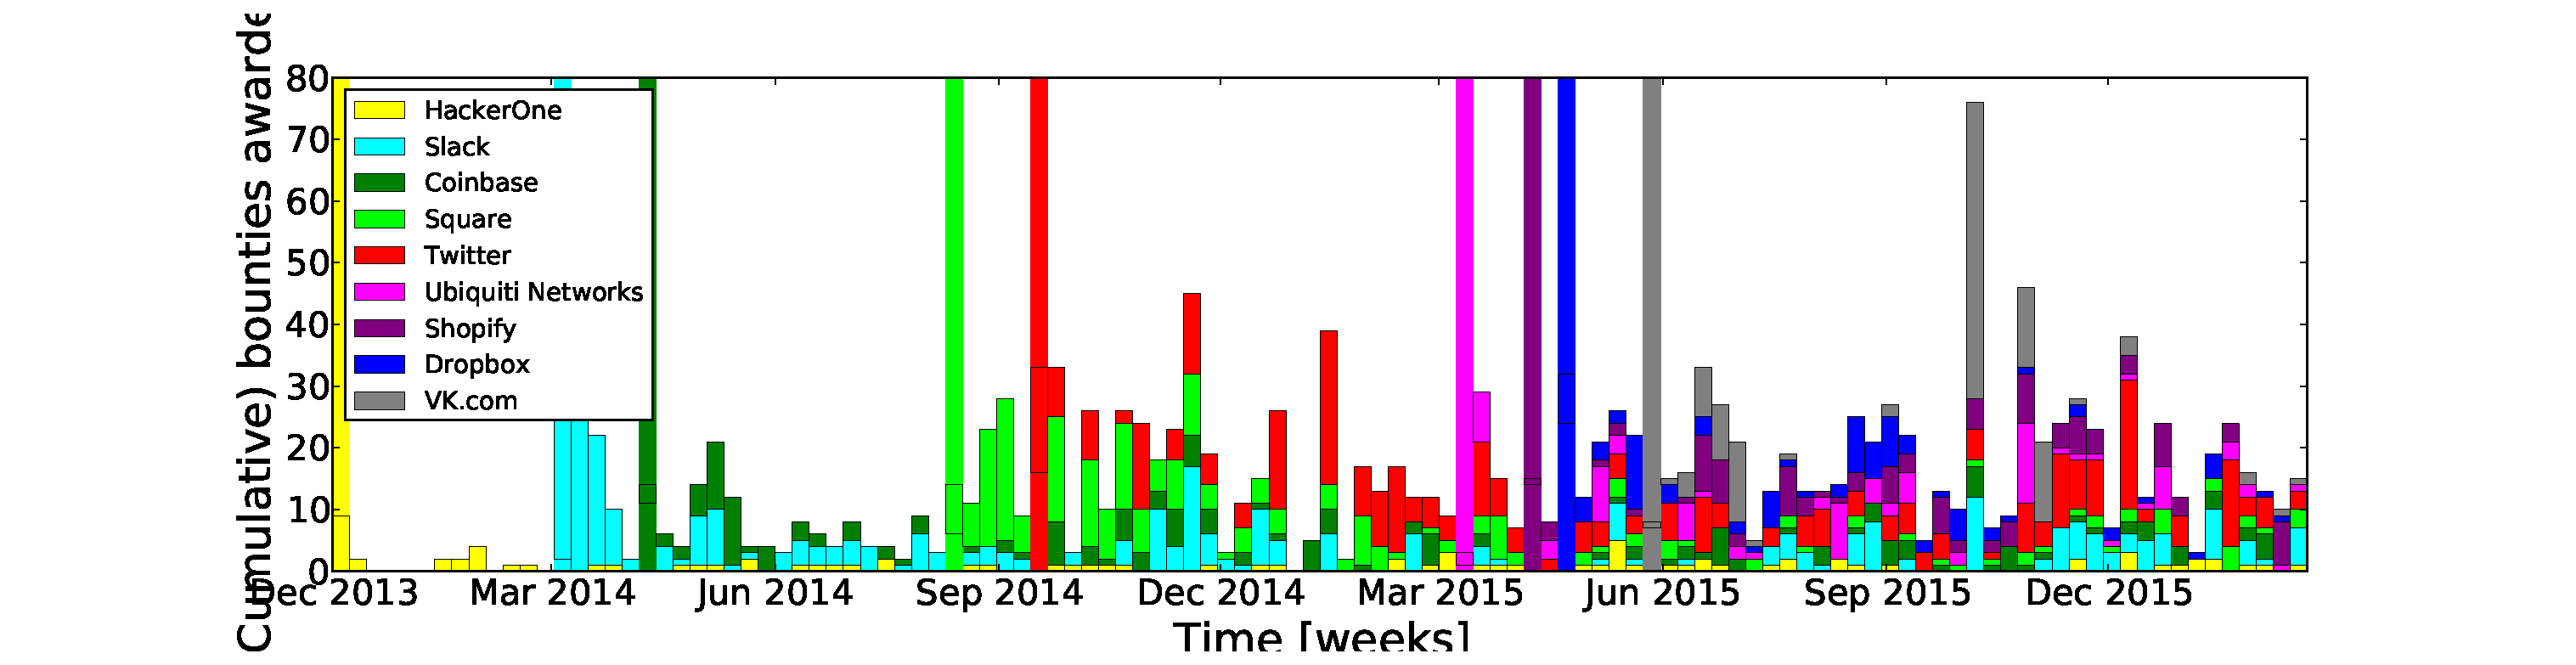
\includegraphics[width=13cm]{figures/timeline.eps}
\caption{{\bf A.} Weekly vulnerability discoveries for the 9 most active programs (with at least 90 bug discoveries as of February 15, 2016). The light colored vertical bars represent the start of the program, occurring when the first bounty is awarded. Most programs exhibit an initial shock (or shortly after the start of the program), followed by a decay of discoveries, which is characterized at the aggregate level by a long-memory process (panel {\bf B}) characterized by a power law decay $\sim t^{\alpha}$ with $\alpha = -0.40(4)$ ($p < 0.001$ and $R^2 = 0.79$) as shown on panel  (for all 35 public programs considered in this study).}
\label{timeline}
\end{center}
\end{figure}



The long-memory process of bug discovery following the launch of a bounty program we observe here, is reminiscent of human timing effects: When the program launches, it takes some time first for the researcher to be exposed (through the media) to the new program, second for the researcher to find and submit bugs, and third for the organization managing the bug bounty program to assess the quality of each submission, and assign a proper bounty reward. To account for all these delays, one may resort to priority queueing applied to humans: First, competing attention prevents immediate exposure to the news of a new program; Second, when security researchers get interested to a new program, they may still be actively searching bugs on other programs or performing other tasks, such as e.g., their regular job, leisure, family matters); Third, when subjected to a flow of bug submissions, security teams at organizations leading bounty programs assign priorities among submissions, and resolve them with human resources available at the time of submission. These delays are best rationalized by human timing contingencies, and moreover, by time as a scare, non-storable resource, and are known to generate long-memory responses of the form $\sim t^{-1.5}$ (in fully rational case) between the arrival and the execution of a task\cite{maillart2011quantification}. The observed much slower decay may result from the compound effect of multiple delays, such as those mentioned above. Since, we consider only the {\it time of discovery} as the moment when the validity of the bug submitted is acknowledged by the program manager, we are mostly blind to the human timing effects associated with the long-memory process observed on Figure \ref{timeline}{\bf B}, including when submissions are made, but don't lead to a discovery (i.e., when the value of the submission is acknowledged by a monetary reward).\\

The initial burst of discoveries, followed by a long-memory decay may also result from the increasing difficulty associated with finding new bugs for each bounty program, as the most obvious vulnerabilities get uncovered first. We thus consider a time-ordered set of bounty rewards $B_p= \{b_1,b_2,b_3,b_k, ..., b_n\}$ for each bounty program $p$, which, on average, maps into a set ordered by difficulty $\widehat{D}$, such that $\widehat{D}(b_{k+1}) > \widehat{D}(b_{k})$.\\
 
The discovery of new bugs in a bounty program is contingent to the number of active security researchers (in the program), and how many vulnerabilities each research is able to find: For a given bounty program, we shall consider the set of bounties $B_{p,r}$ associated with bugs found by researcher $r$.\\

We also investigate how the launch of a new bounty program is likely to create a new windfall effect, hence attracting researchers currently busy searching bugs in already existing bounty programs


{\bf some researchers may be actually groups of security researchers (e.g., a whole security consulting company)}




\section{Method}
\label{sec:method}
Bug bounty programs work on the premise that humans as a crowd are efficient at searching and finding bugs. Their mere existence is a {\it de facto} recognition that market approaches for bug discovery bring efficiency, beyond in-house security. Bug bounty programs signal that organizations are ready to complement their vertical cost-effective security operations with market approaches, which are traditionally perceived as less cost-effective, yet more adaptive \cite{coase1937}. Early on, Brady et al. \cite{brady1999murphy} have offered a hint for the existence of such markets for bugs: according to their proposed theory, each researcher has slightly different skills and mindset. When a security researcher tests a software piece by choosing the inputs, she offers a unique operational environment. This environment is prone to the discovery of new bugs, which may not have been seen by other researchers. The proposed theory by Brady et al. \cite{brady1999murphy} intrinsically justifies the existence of bug bounty program structures as markets, which provide the necessary diversity to account for the highly uncertain risk horizon of bug discovery. Here, we develop a quantitative method to formalize a mechanism and to test the theory proposed in \cite{brady1999murphy}. This validation step shall help provide organizational design insights for bug bounty programs.\\

For that, we investigate the interplay between the vulnerability discovery process and the cumulative rewards distributed to security researchers within and across 35 public bounty programs hosted on HackerOne. When a bug bounty program starts, it attracts a number of security researchers, who in turn submit bugs. Subsequent bug discoveries get increasingly difficult for each individual researcher, and to some extent for all researchers together. The difficulties faced by security researchers can be technical. They can also be the result of insufficient or conflicting incentives. Here, we develop and test a model, which accounts for both technical difficulties and insufficient incentives. We further address conflicting incentives by measuring the effect of newly launched bug bounty programs on incumbent programs.\\

Starting from an initial probability of discovering the first vulnerability $P(k=0) = 1$, the probability to find a second bug is a fraction of the former probability: $P_{k+1} = \beta * P_k$ with $\beta$ a constant strictly smaller than one. The probability that no more discoveries will be made after $k$ steps is given by $P_k = \beta^{k} (1-\beta)$. Conversely, starting from the initial reward $R_0 = R(k=0)$, the subsequent reward $R_1 = \Lambda_1 \cdot R_0$, and further additional reward $ R_2 = \Lambda_2 \Lambda_1 \cdot R_{0}$. After $n$ steps, the total reward is the sum of all past rewards: 

\begin{equation}
R_{n} = R_{0} \sum_{k=1}^{n} \Lambda_1 ... \Lambda_k.
\end{equation}

Thus, $R_{n}$ is the recurrence solution of the  
Kesten map ($R_{n} = \Lambda_n R_{n-1} +R_0$)
\cite{kesten1973random,sornette1997convergent}:  as soon as amplification occurs (technically, 
some of the factors $\Lambda_k$ are larger than $1$), the distribution
of rewards is a power law, whose exponent $\mu$ is a function of $\beta$
and of the distribution of the factors $\Lambda_k$. In the case where
all factors are equal to $\Lambda$, this model predicts three possible regimes for the distribution of rewards (for a given program): thinner than exponential for $\Lambda < 1$, exponential for $\Lambda = 1$, and power law for $\Lambda > 1$ with exponent $\mu = |\ln \beta|/ \ln \Lambda$ (see Appendix). The expected payoff of vulnerability discovery is given by,

\begin{equation}
\label{ }
U_k = P_k \times R_k,
\end{equation}

\noindent with both $P_k$ and $R_k$ random variables respectively determined by $\beta$ and $\Lambda$. Because $U_k$ is a multiplication of diverging probability and reward components, its nature is reminiscent of the St. Petersburg paradox (or St. Petersburg lottery), proposed first by the Swiss Mathematician Nicolas Bernoulli in 1713, and later formalized by his brother Daniel in 1738 \cite{bernoulli1954exposition}.  The St. Petersburg paradox states the problem of decision-making when both the probability and the reward are diverging  for $k \rightarrow \infty$: a player has a chance to toss a fair coin at each stage of the game. The pot starts at two and is doubled every time a head appears. The first time a tail appears, the game ends and the player wins whatever is in the pot. Thus the player wins two if a tail appears on the first toss, four if a head appears on the first toss and a tail on the second, eight if a head appears on the first two tosses and a tail on the third, and so on. The main interest of Bernoulli was to determine how much a player would be ready to pay for this game, and he found that very few people would like to play this game even though the expected utility increases (in the simplest case proposed by Bernoulli, $U_n = \sum_{k=0}^{n} U_k = n$) \cite{bernoulli1954exposition}. The situation of a security researcher differs from the St. Petersburg lottery as bug search costs are incurred at every step. Since these costs influence the probability to find an additional bug, the cost can be at least partially integrated in $P_k$. We could assume equivalently that costs are integrated into the utility as $U^{*}_k = U_k - c_k$. Here, we don't factor these costs in because their exact nature is largely undetermined and our data don't offer a reliable proxy. The security researcher may also decide to stop searching for bugs in a program, at any time $k$. This is equivalent to setting $P_{k+1} = 0$.\\

The expected payoff $U_k$ therefore determines the incentive structure for security researchers, given that the bounty program manager can tune $R_0$ and to some extent $\Lambda$. The utility function may also incorporate non-monetary incentives, such as reputation: finding a long series of bugs may signal some fitness for a bug bounty program and  thus create a permanent job opportunity \cite{moussouris2016}. Similarly, discovery of a rare (resp. critical) bug that no other researcher has found before has a strong signaling effect, which can help make a career. However, these strategies are high-risk high-return. Therefore, they carry additional fame. In the next section, we will calibrate our model to the bug discovery process associated with 35 bounty programs publicly documented on the HackerOne platform.

 %However, rules are generally set upfront and shall not be changed in the course of the bounty program. Changing game rules is risky as it may undermine trust in the program. Here, we assume that bounty program managers don't tune their reward policy after the bug bounty program has started. 

%\sout{In principle, the manager could set $R_0$ to influence $P_0$ and indirectly $P_{k}$. Mapping the discovery rank $k$ into the rate of discovery may also help considering discounting aspects in presence of competing opportunities and inter-temporal choices under uncertainty \cite{loewenstein1992anomalies}. A new public bounty program is launched at a Poisson rate, approximately every 2 months, and each launch brings its windfall effect, leaving the researcher with the choice to either keep digging increasingly harder vulnerabilities (rare but with higher reward), or turning to the low hanging fruit (frequent but with low reward) of a new program. We shall therefore verify whether newly launched programs actually influence security researchers.}


%The propensity for security researchers to keep searching for vulnerabilities is conditioned by the trend of $U(k)$: if $U \rightarrow 0$ when $k \rightarrow \infty$, then it's likely that they will leave the program (it's a bit sketchy here). If do not consider the costs (i.e., effort spent on finding the $k^{th}$ bug, which we cannot measure here (see next subsection on timing effects), but which is indirectly captured by $P(k)$), then in the presence of a variety of programs at different stages of their life (i.e., at different values of $k$), the security researcher is left with comparing utility between programs.

%\begin{figure}
%\begin{center}
%%\includegraphics[width=10cm]{figures/decay.eps}
%\caption{Distribution of discovery waiting time between ranks $\rightarrow$ the hope is to find that time increases as $k \rightarrow \infty$.}
%\label{fig:decay}
%\end{center}
%\end{figure}



%The incentive mechanism is then completely driven by the probability of discovery of the $k+1$ vulnerability given that $k$ bugs have already been discovered on the one hand, and by the expected reward for the $k+1$ discovery on the other hand. When the probability of finding a bug decreases fast while the reward for a new bug increases fast, in such a way that the product $f_k \times R_k$ remains constant, then the expected value of the game increases linearly as $k \rightarrow \infty$. This problem is reminiscent 


%When a bug bounty program (by an organization) is launched immediate vulnerabilities are found by security researchers and rewarded by organizations. The cost of finding a new vulnerability increases as more discoveries occur, and thus, incentives should be set accordingly to keep onboard security researchers, or at least, the best researchers who have the capabilities to find increasingly subtle problems. 



%Searching for bugs in software is an attrition process: When the search starts, obvious bugs are found first. Subsequent bug discoveries get increasingly difficult. When a bug bounty program (by an organization) is launched immediate vulnerabilities are found by security researchers and rewarded by organizations. The cost of finding a new vulnerability increases as more discoveries occur, and thus, incentives should be set accordingly to keep onboard security researchers, or at least, the best researchers who have the capabilities to find increasingly subtle problems. 
%
%{\bf aim 1:} understand the evolution of expected utility of security researchers as an increasing amount of vulnerabilities get discovered for a given program. And how the incentive mechanism varies from one program to another\\
%
%{\bf aim 2:} understand how bug bounties compete with each others? Each time, a new bug bounty program is launched, a new set of opportunities arises, and security researchers must make a choice (though not a binary choice) between digging further in an existing program (with lower probability to find a vulnerability, but presumably with higher utility) or turning to a new program (with higher probability to find a vulnerability, but presumably with lower utility).
%
%{\bf aim3: } What can we say about the whole eco-system?



\section{results}

\begin{figure}
\begin{center}
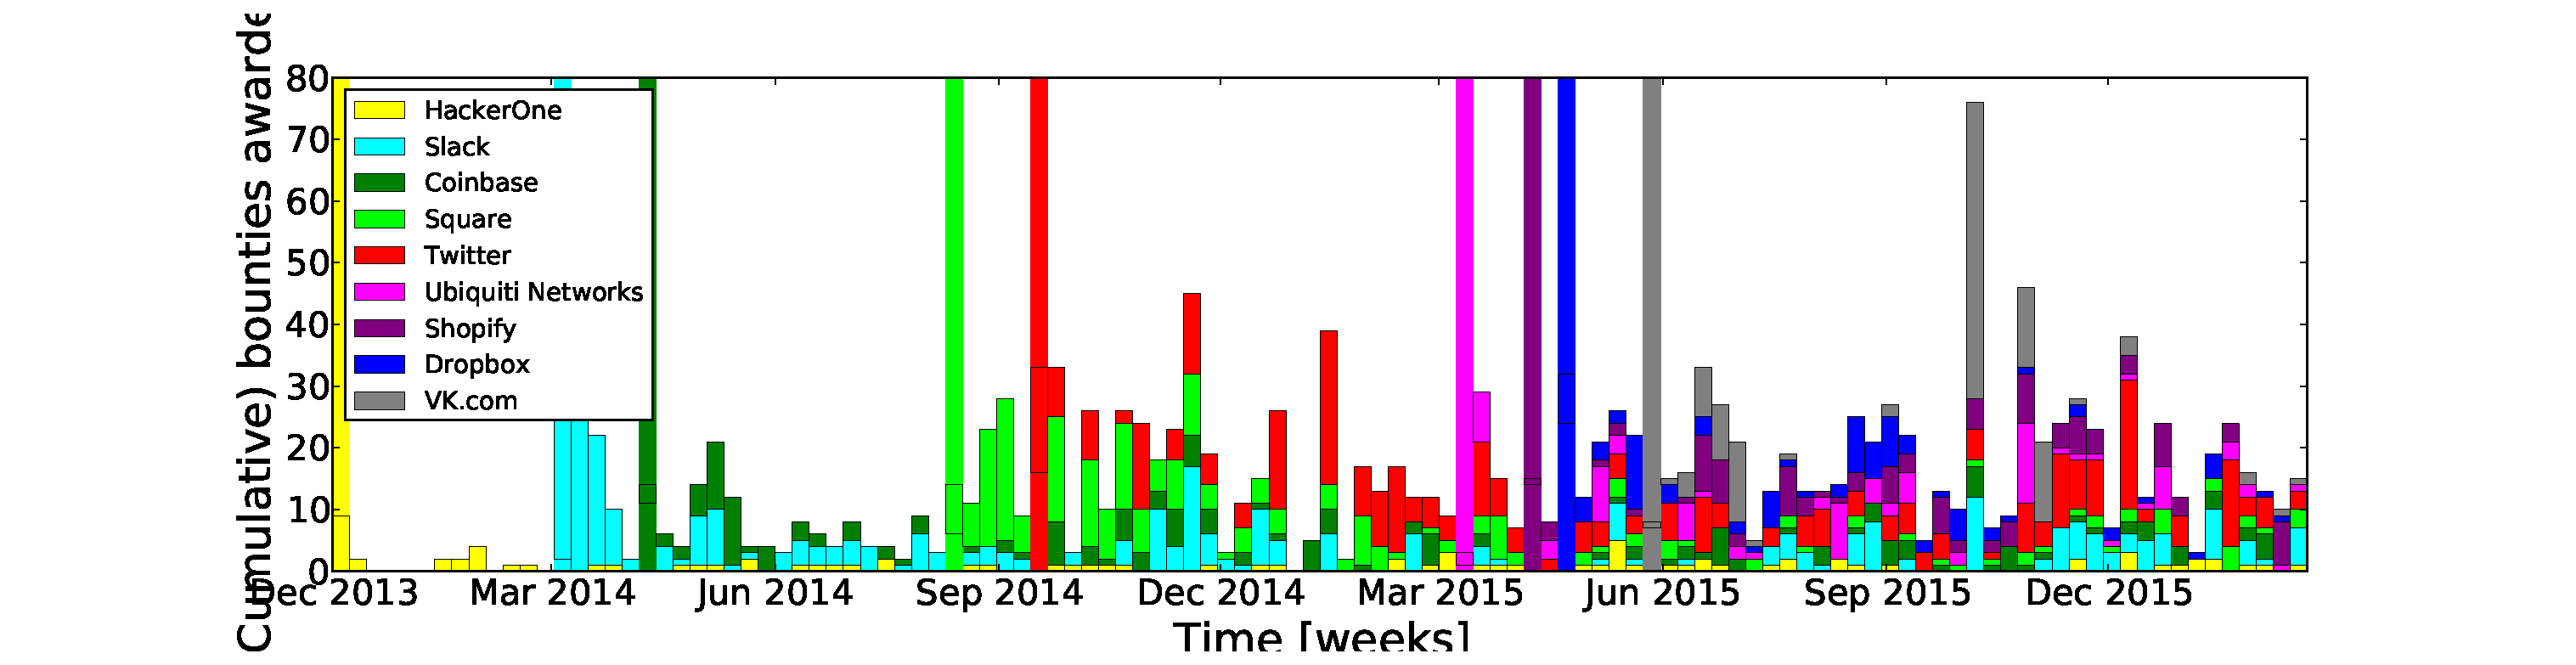
\includegraphics[width=16cm]{figures/timeline.eps}
\caption{ }
\label{ }
\end{center}
\end{figure}


\begin{figure}
\begin{center}
\includegraphics[width=10cm]{figures/density_joining.eps}
\caption{ }
\label{ }
\end{center}
\end{figure}



{\bf Scaling bugs as a function of researchers per program:}
\begin{equation}
R \sim c^{\beta}
\end{equation}

with $\beta \approx 1.13$ (see Figure \ref{fig:scaling}).


\begin{figure}
\begin{center}
\includegraphics[width=10cm]{figures/scaling_bugs_vs_researchers.eps}
\caption{ }
\label{fig:scaling}
\end{center}
\end{figure}





Let us call $\{R_1, R_2, ..., R_{c-1}, R_c\}$, the total number of bugs found respectively by security researchers $1, 2, ..., c-1, c$. 
Let us call $R_{\rm max}(c)$, the largest among the set  $\{R_1, R_2, ..., R_{c-1}, R_c\}$. A good estimate of $R_{\rm max}(c)$ is obtained by the condition that the probability $\int_{R_{\rm max}(c)}^{+\infty}  p(r) dr$ to find a security researcher with a total contribution equal to or larger than $R_{\rm max}(c)$ times the number $c$ of active developers is equal to $1$, i.e., by the definition of $R_{\rm max}(c)$, there should be typically only one 
security researcher with such a number of bugs found. This yields
\be
 R_{\rm max}(c)  \sim c^{1/\mu} ~. 
 \label{sdfjhsg9e}
\ee



An estimate of the typical total number of bugs  $R_1 +  R_2 + ... + R_c$  identified
by the $c$ security researchers can  then be obtained as  \cite{Bougeorges,sornette2006critical}
\be
R_1 +  R_2 + ... + R_c   \approx c  \int_0^{R_{\rm max}(c)} r   p(r) dr
 \sim  c^{1/\mu}    ~,~~~~{\rm  for}~\mu <1~.
 \label{rjtik6ik}
\ee


We stress that the scaling $\sim c^{1/\mu}$ only holds for $\mu <1$ and is replaced
by $\sim c$, i.e., linearity, for $\mu > 1$.
The upper bound in the integral in (\ref{rjtik6ik}) reflects that
the random variables $\{R_1, R_2, ..., R_{c-1}, R_c\}$ are not larger than $R_{\rm max}(c)$
by definition of the later. According to equation (\ref{rjtik6ik}), the typical
total production (number of commits) by $c$ developers
is proportional to $c^{1/\mu}$, when their contributions are wildly distributed
with a power law distribution with exponent $\mu <1$. According to this large
deviation mechanism, the superlinear exponent $\beta$ is equal to $1/\mu$.
\be
{\rm \bf prediction~of ~the~ large~ deviation ~mechanism}: ~\beta = 1/\mu~, ~{\rm for}~\mu < 1~.
\label{eyyn}
\ee

Within this large deviation mechanism, explaining the superlinear productive activity ($\beta>1$) 
reduces to explaining the heavy-tailed distribution of commits $R$ per contributor over a large period of time,
i.e., amounts to derive the power law distribution (\ref{srthyjueyt}) with $\mu <1$. For this, the next section
proposes a generic model.


\be
{\rm \bf prediction~of ~the~ large~ deviation ~mechanism}: ~\beta = 1/\mu~, ~{\rm for}~\mu < 1~.
\label{eyyn}
\ee


Distribution of bugs found per programmer per program:
\begin{equation}
P(X > x) = 1/x^{\alpha},~with~\gamma = 1.60(7) 
\end{equation}

{\bf Distribution of bugs per program:}
\begin{equation}
P^{tot}_{>}(R > r) = 1/x^{\mu},~with~\mu = 0.8(4) 
\end{equation}

Distribution of researchers per program:
\begin{equation}
P(X > x) = 1/x^{\gamma},~with~\alpha = 0.9(5) 
\end{equation}



{\bf mapping}

- superlinear exponent (same)\\
- bug bounty program  $\Leftrightarrow$ OSS contributor \\










\begin{figure}
\begin{center}
\includegraphics[width=16cm]{figures/ccdfs.png}
\caption{ }
\label{ }
\end{center}
\end{figure}
\section{Discussion}
\label{sec:discussion}


\subsection{Timing effects}

What if not only the probability to find a vulnerability decreases, but it takes an increasing amount of time? 



Limited information on time between vulnerability submission and 


\subsection{public versus private programs}


\subsection{Renewal as code changes}



{\bf Is it bad or good if a researcher submits a duplicate bug?  It's probably bad, but still the learning component remains ? (in relation to all-pay auctions?)}



{\bf Correlation between reputation and capacity to discover bugs with high rank ?}

{\bf Cascades, learning, re-inforcing process}

{\bf our results suggest that program managers should enroll a lot of security researchers early on, if not before the start of the program, to maximize the initial pool of researchers who in turn can compound best on their cumulative knowledge i.e., $t^{1.4 - 1.27}$}

{\bf now bounty program managers face a tradeoff: the more the initial load, the longer the response time in order to go through all submissions (show evidence)}

{\bf strange thing: on the contrary of usual crowdsourcing, here the security researcher has access to the same information as the user of the software platform.}


{\bf it remains to be explained the distribution of number of vulns discovered per participant: critical cascades?}



\cite{benkler2011penguin}

We present a model of workers supplying labor to paid crowdsourcing projects. We also introduce a novel method for estimating a worker's reservation wage - the key parameter in our labor supply model. We tested our model by presenting experimental subjects with real-effort work scenarios that varied in the offered payment and difficulty. As predicted, subjects worked less when the pay was lower. However, they did not work less when the task was more time-consuming. Interestingly, at least some subjects appear to be "target earners," contrary to the assumptions of the rational model. The strongest evidence for target earning is an observed preference for earning total amounts evenly divisible by 5, presumably because these amounts make good targets. Despite its predictive failures, we calibrate our model with data pooled from both experiments. We find that the reservation wages of our sample are approximately log normally distributed, with a median wage of \$1.38/hour. We discuss how to use our calibrated model in applications. \cite{horton2010labor}


\section{Conclusion}
\label{sec:conclusion}
In this paper, we have investigated how crowds of security researchers hunt software bugs and vulnerabilities and report to a bug bounty platform. Consistent with the famous adage ``Given enough eyeballs, all bugs are shallow" by Eric Raymond \cite{raymond1999cathedral}, we have found that security researchers face challenging difficulties when trying to uncover large numbers of bugs in a same bounty program: The super-linear reward increase for each new bug found does not counterbalance the sharply decreasing probability of finding new bugs by the same person. This result is consistent with the theory proposed by Brady et al. on maximized entropy of bug discovery as an evolutionary process, following adaptation to changing environments \cite{brady1999murphy}: Each security researcher tests software within an environment bounded by her skills and mindset. This result brings a fundamental justification for the existence of markets for bugs, beyond internalized security operations and research: Bug bounty programs offer a way to capitalize on these {\it environments} provided by the involvement of many security researchers. Yet difficulties for researchers to find large numbers of bugs in one bug bounty program bring incentives for mobility across programs. In particular, we find that the launch of new bug bounty programs has a negative effect on incumbent programs regarding bug submissions. We thus bring forth 3 organization design recommendations. First, mobility shall be encouraged across bug bounty programs and perhaps across bug bounty platforms. Second, one major duty of bug bounty platforms shall be to enroll large number of security researchers, and guide them towards low-hanging fruits, which for new researchers, may not necessarily be new bug bounty programs. Finally, bug bounty program manager shall feature significant changes in the codebase, such as major releases, to help security researchers focus on issues they have not been exposed previously. Such strategy shall help retain more long-term engagement, while not crowding out motivation in face of difficulty. 


%\subsubsection*{Acknowledgements}
%\acknowledgements{This research was supported in part by the National Science Foundation through award CCF-0424422 (TRUST - Team for Research in Ubiquitous Secure Technology). One of the authors (TM) acknowledges support from the Swiss National Science Foundation (SNSF; Grants PA00P2\_145368  and P300P2\_158462). The authors would like to thank Aron Laszka for his valuable comments, as well as the 3 anonymous reviewers who provided insightful comments and thus contributed to a considerable improvement of the manuscript.}

\bibliographystyle{apsrev4-1}
\bibliography{../references}

\end{document}




 


